% ============================================================
% Question Bank: ch05-01 Writing Two-Step Equations from Word Problems
% Topic Title: Writing Two-Step Equations from Word Problems
% CCSS: 7.EE.B.4.A
% Questions: 30 (18 MC + 7 SA + 5 Graphical)
% ============================================================

% --- Multiple Choice Questions (18) ---

\begin{practiceQuestion}{5-1-q01}{mc}
\begin{questionText}
A movie ticket costs $\$d$ each. You buy $4$ tickets and a $\$6$ popcorn combo. The total is $\$42$. Which equation represents this situation?
\end{questionText}
\choiceA{$4d - 6 = 42$}
\choiceB{$4d + 6 = 42$}
\choiceC{$6d + 4 = 42$}
\choiceD{$4 + 6d = 42$}
\correctAnswer{B}
\explanation{$4$ tickets at $\$d$ each is $4d$, plus $\$6$ popcorn: $4d + 6 = 42$.}
\end{practiceQuestion}

\begin{practiceQuestion}{5-1-q02}{mc}
\begin{questionText}
``Seven times a number plus $3$ equals $52$.'' Which equation matches this statement?
\end{questionText}
\choiceA{$7 + 3n = 52$}
\choiceB{$7(n + 3) = 52$}
\choiceC{$7n + 3 = 52$}
\choiceD{$3n + 7 = 52$}
\correctAnswer{C}
\explanation{``Seven times a number'' is $7n$. ``Plus $3$'' gives $7n + 3$. ``Equals $52$'' gives $7n + 3 = 52$.}
\end{practiceQuestion}

\begin{practiceQuestion}{5-1-q03}{mc}
\begin{questionText}
A bike shop charges $\$15$ per hour for rentals plus a $\$10$ helmet fee. Maria's total bill is $\$55$. Which equation can be used to find the number of hours $h$ she rented the bike?
\end{questionText}
\choiceA{$15h - 10 = 55$}
\choiceB{$10h + 15 = 55$}
\choiceC{$15 + 10h = 55$}
\choiceD{$15h + 10 = 55$}
\correctAnswer{D}
\explanation{The rental cost is $15h$ and the helmet fee is $\$10$: $15h + 10 = 55$.}
\end{practiceQuestion}

\begin{practiceQuestion}{5-1-q04}{mc}
\begin{questionText}
You have $\$80$ and spend $\$12$ per week. After $w$ weeks, you have $\$20$ left. Which equation models this situation?
\end{questionText}
\choiceA{$80 + 12w = 20$}
\choiceB{$80 - 12w = 20$}
\choiceC{$12w - 80 = 20$}
\choiceD{$80w - 12 = 20$}
\correctAnswer{B}
\explanation{Start with $\$80$, subtract $\$12$ each week: $80 - 12w = 20$.}
\end{practiceQuestion}

\begin{practiceQuestion}{5-1-q05}{mc}
\begin{questionText}
A school fundraiser sells candles for $\$8$ each. The class already raised $\$45$ from a bake sale. They need a total of $\$125$. Which equation finds the number of candles $c$ they must sell?
\end{questionText}
\choiceA{$8c - 45 = 125$}
\choiceB{$45c + 8 = 125$}
\choiceC{$8c + 45 = 125$}
\choiceD{$8 + 45c = 125$}
\correctAnswer{C}
\explanation{Candle sales bring in $8c$, plus the $\$45$ already raised: $8c + 45 = 125$.}
\end{practiceQuestion}

\begin{practiceQuestion}{5-1-q06}{mc}
\begin{questionText}
``A number divided by $5$, then increased by $8$, equals $20$.'' Which equation matches?
\end{questionText}
\choiceA{$\dfrac{n}{5} - 8 = 20$}
\choiceB{$\dfrac{n + 8}{5} = 20$}
\choiceC{$5n + 8 = 20$}
\choiceD{$\dfrac{n}{5} + 8 = 20$}
\correctAnswer{D}
\explanation{``A number divided by $5$'' is $\frac{n}{5}$. ``Increased by $8$'' gives $\frac{n}{5} + 8$. ``Equals $20$'' gives $\frac{n}{5} + 8 = 20$.}
\end{practiceQuestion}

\begin{practiceQuestion}{5-1-q07}{mc}
\begin{questionText}
A plumber charges $\$50$ for a house call plus $\$35$ per hour. The total bill is $\$190$. Which equation can be used to find the number of hours $h$ the plumber worked?
\end{questionText}
\choiceA{$50h + 35 = 190$}
\choiceB{$35h + 50 = 190$}
\choiceC{$50 - 35h = 190$}
\choiceD{$85h = 190$}
\correctAnswer{B}
\explanation{The hourly charge is $35h$, plus the $\$50$ house call: $35h + 50 = 190$.}
\end{practiceQuestion}

\begin{practiceQuestion}{5-1-q08}{mc}
\begin{questionText}
An elevator starts at floor $3$ and goes up $2$ floors every minute. After $m$ minutes it is at floor $15$. Which equation represents this?
\end{questionText}
\choiceA{$3m + 2 = 15$}
\choiceB{$2m - 3 = 15$}
\choiceC{$2m + 3 = 15$}
\choiceD{$15 - 2m = 3$}
\correctAnswer{C}
\explanation{Starts at floor $3$, rises $2$ floors per minute: $2m + 3 = 15$.}
\end{practiceQuestion}

\begin{practiceQuestion}{5-1-q09}{mc}
\begin{questionText}
``Three less than twice a number is $17$.'' Which equation matches this statement?
\end{questionText}
\choiceA{$3 - 2n = 17$}
\choiceB{$2n - 3 = 17$}
\choiceC{$2(n - 3) = 17$}
\choiceD{$2n + 3 = 17$}
\correctAnswer{B}
\explanation{``Twice a number'' is $2n$. ``Three less than'' means subtract $3$: $2n - 3 = 17$.}
\end{practiceQuestion}

\begin{practiceQuestion}{5-1-q10}{mc}
\begin{questionText}
A cell phone plan costs $\$0.10$ per text message plus $\$25$ per month. Last month's bill was $\$37$. Which equation can find the number of texts $t$?
\end{questionText}
\choiceA{$25t + 0.10 = 37$}
\choiceB{$0.10t - 25 = 37$}
\choiceC{$0.10t + 25 = 37$}
\choiceD{$35t = 37$}
\correctAnswer{C}
\explanation{Each text costs $\$0.10$, so $t$ texts cost $0.10t$. Add the $\$25$ monthly fee: $0.10t + 25 = 37$.}
\end{practiceQuestion}

\begin{practiceQuestion}{5-1-q11}{mc}
\begin{questionText}
A swimming pool is being drained at a rate of $50$ gallons per hour. The pool currently has $1{,}200$ gallons. After $h$ hours, $200$ gallons remain. Which equation models this?
\end{questionText}
\choiceA{$50h + 200 = 1{,}200$}
\choiceB{$1{,}200 + 50h = 200$}
\choiceC{$1{,}200 - 50h = 200$}
\choiceD{$200 - 50h = 1{,}200$}
\correctAnswer{C}
\explanation{Start with $1{,}200$ gallons and remove $50$ gallons per hour: $1{,}200 - 50h = 200$.}
\end{practiceQuestion}

\begin{practiceQuestion}{5-1-q12}{mc}
\begin{questionText}
Which situation could be modeled by the equation $6x + 15 = 57$?
\end{questionText}
\choiceA{You earn $\$6$ per hour and already have $\$15$. You want $\$57$ total.}
\choiceB{You buy $15$ items at $\$6$ each and pay $\$57$ tax.}
\choiceC{You spend $\$6$ plus $\$15$ for a total of $\$57$.}
\choiceD{You buy $6$ items for $\$57$ and get $\$15$ change.}
\correctAnswer{A}
\explanation{Earning $\$6$ per hour for $x$ hours gives $6x$, plus the $\$15$ already saved: $6x + 15 = 57$.}
\end{practiceQuestion}

\begin{practiceQuestion}{5-1-q13}{mc}
\begin{questionText}
A carpenter has a board that is $96$ inches long. He cuts off pieces that are $x$ inches long. After cutting $8$ pieces, he has $16$ inches left. Which equation can be used to find $x$?
\end{questionText}
\choiceA{$96 + 8x = 16$}
\choiceB{$8x - 96 = 16$}
\choiceC{$96 - 8x = 16$}
\choiceD{$96 - 16x = 8$}
\correctAnswer{C}
\explanation{Start with $96$ inches, remove $8$ pieces of $x$ inches each: $96 - 8x = 16$.}
\end{practiceQuestion}

\begin{practiceQuestion}{5-1-q14}{mc}
\begin{questionText}
``Twelve more than four times a number is $44$.'' What is the equation?
\end{questionText}
\choiceA{$12n + 4 = 44$}
\choiceB{$4n + 12 = 44$}
\choiceC{$4(n + 12) = 44$}
\choiceD{$4n - 12 = 44$}
\correctAnswer{B}
\explanation{``Four times a number'' is $4n$. ``Twelve more than'' means add $12$: $4n + 12 = 44$.}
\end{practiceQuestion}

\begin{practiceQuestion}{5-1-q15}{mc}
\begin{questionText}
A parking garage charges $\$3$ per hour after a flat fee of $\$5$. You paid $\$23$. Which equation finds the number of hours $h$ you parked?
\end{questionText}
\choiceA{$5h + 3 = 23$}
\choiceB{$3h - 5 = 23$}
\choiceC{$3h + 5 = 23$}
\choiceD{$8h = 23$}
\correctAnswer{C}
\explanation{Hourly charge: $3h$, plus the flat fee: $3h + 5 = 23$.}
\end{practiceQuestion}

\begin{practiceQuestion}{5-1-q16}{mc}
\begin{questionText}
Which equation represents ``nine less than a number divided by $2$ is $7$''?
\end{questionText}
\choiceA{$\dfrac{n}{2} + 9 = 7$}
\choiceB{$\dfrac{n - 9}{2} = 7$}
\choiceC{$\dfrac{n}{2} - 9 = 7$}
\choiceD{$9 - \dfrac{n}{2} = 7$}
\correctAnswer{C}
\explanation{``A number divided by $2$'' is $\frac{n}{2}$. ``Nine less than'' means subtract $9$: $\frac{n}{2} - 9 = 7$.}
\end{practiceQuestion}

\begin{practiceQuestion}{5-1-q17}{mc}
\begin{questionText}
A dog walker earns $\$7$ per dog plus a $\$20$ tip. She earned $\$55$ today. Which equation finds the number of dogs $d$ she walked?
\end{questionText}
\choiceA{$20d + 7 = 55$}
\choiceB{$7d - 20 = 55$}
\choiceC{$7d + 20 = 55$}
\choiceD{$27d = 55$}
\correctAnswer{C}
\explanation{Walking $d$ dogs at $\$7$ each is $7d$, plus $\$20$ tip: $7d + 20 = 55$.}
\end{practiceQuestion}

\begin{practiceQuestion}{5-1-q18}{mc}
\begin{questionText}
A tank has $500$ liters of water. A hose adds $25$ liters per minute. After $m$ minutes the tank has $750$ liters. Which equation is correct?
\end{questionText}
\choiceA{$500 - 25m = 750$}
\choiceB{$25m - 500 = 750$}
\choiceC{$500 + 25m = 750$}
\choiceD{$25m + 750 = 500$}
\correctAnswer{C}
\explanation{Start with $500$ liters and add $25$ liters per minute: $500 + 25m = 750$.}
\end{practiceQuestion}

% --- Short Answer Questions (7) ---

\begin{practiceQuestion}{5-1-q19}{sa}
\begin{questionText}
Write an equation: ``You buy $n$ books at $\$6$ each and pay $\$4$ for shipping. The total cost is $\$34$.''
\end{questionText}
\correctAnswer{$6n + 4 = 34$}
\explanation{$n$ books at $\$6$ each is $6n$, plus $\$4$ shipping: $6n + 4 = 34$.}
\end{practiceQuestion}

\begin{practiceQuestion}{5-1-q20}{sa}
\begin{questionText}
A baker makes $c$ cakes per day. After $5$ days, she donates $10$ cakes and has $40$ cakes left. Write an equation to find $c$.
\end{questionText}
\correctAnswer{$5c - 10 = 40$}
\explanation{In $5$ days she makes $5c$ cakes. After donating $10$: $5c - 10 = 40$.}
\end{practiceQuestion}

\begin{practiceQuestion}{5-1-q21}{sa}
\begin{questionText}
Write an equation for: ``Twice a number, decreased by $11$, is $-3$.''
\end{questionText}
\correctAnswer{$2n - 11 = -3$}
\explanation{``Twice a number'' is $2n$. ``Decreased by $11$'' gives $2n - 11$. ``Is $-3$'' gives $2n - 11 = -3$.}
\end{practiceQuestion}

\begin{practiceQuestion}{5-1-q22}{sa}
\begin{questionText}
A car rental company charges $\$40$ per day plus $\$0.15$ per mile. A customer paid $\$67$ for one day. Write an equation to find the number of miles $m$ driven.
\end{questionText}
\correctAnswer{$0.15m + 40 = 67$}
\explanation{The mileage cost is $0.15m$, plus the daily fee of $\$40$: $0.15m + 40 = 67$.}
\end{practiceQuestion}

\begin{practiceQuestion}{5-1-q23}{sa}
\begin{questionText}
A thermometer reads $-4\degree$F. The temperature rises $t$ degrees each hour. After $3$ hours it reads $14\degree$F. Write an equation for $t$.
\end{questionText}
\correctAnswer{$3t + (-4) = 14$ or $3t - 4 = 14$}
\explanation{Start at $-4$ and add $t$ degrees for $3$ hours: $-4 + 3t = 14$, or equivalently $3t - 4 = 14$.}
\end{practiceQuestion}

\begin{practiceQuestion}{5-1-q24}{sa}
\begin{questionText}
Write an equation for: ``A number divided by $3$, plus $7$, equals $15$.''
\end{questionText}
\correctAnswer{$\dfrac{n}{3} + 7 = 15$}
\explanation{``A number divided by $3$'' is $\frac{n}{3}$. ``Plus $7$'' gives $\frac{n}{3} + 7$. ``Equals $15$'' gives $\frac{n}{3} + 7 = 15$.}
\end{practiceQuestion}

\begin{practiceQuestion}{5-1-q25}{sa}
\begin{questionText}
You owe your friend $\$50$. You pay back $\$8$ per week. After $w$ weeks you still owe $\$18$. Write an equation.
\end{questionText}
\correctAnswer{$50 - 8w = 18$}
\explanation{Start owing $\$50$, pay $\$8$ each week: $50 - 8w = 18$.}
\end{practiceQuestion}

% --- Graphical Questions (3 GMC + 2 GSA) ---

\begin{practiceQuestion}{5-1-q26}{gmc}
\begin{questionText}
The diagram below shows a balance scale. Which equation represents the balance?

\begin{center}
\begin{tikzpicture}[scale=0.8]
  % Fulcrum
  \draw[thick] (0,-0.5) -- (-0.4,-1.2) -- (0.4,-1.2) -- cycle;
  % Beam
  \draw[thick] (-4,0) -- (4,0);
  % Left pan
  \draw[thick] (-4,0) -- (-4.5,-0.5) -- (-3.5,-0.5) -- (-4,0);
  \draw[thick,fill=funBlue!20] (-4.5,-0.5) -- (-4.5,-0.8) -- (-3.5,-0.8) -- (-3.5,-0.5) -- cycle;
  \node at (-4,-0.65) {$3x + 5$};
  % Right pan
  \draw[thick] (4,0) -- (4.5,-0.5) -- (3.5,-0.5) -- (4,0);
  \draw[thick,fill=funOrange!20] (3.5,-0.5) -- (3.5,-0.8) -- (4.5,-0.8) -- (4.5,-0.5) -- cycle;
  \node at (4,-0.65) {$26$};
\end{tikzpicture}
\end{center}
\end{questionText}
\choiceA{$3x - 5 = 26$}
\choiceB{$5x + 3 = 26$}
\choiceC{$3x + 5 = 26$}
\choiceD{$3(x + 5) = 26$}
\correctAnswer{C}
\explanation{The left pan shows $3x + 5$ and the right pan shows $26$. The balance means $3x + 5 = 26$.}
\end{practiceQuestion}

\begin{practiceQuestion}{5-1-q27}{gmc}
\begin{questionText}
The table below shows the cost of concert tickets. Which equation represents the total cost $C$ for $t$ tickets?

\begin{center}
\begin{tabular}{|c|c|}
\hline
\textbf{Tickets ($t$)} & \textbf{Total Cost ($C$)} \\
\hline
$1$ & $\$17$ \\
\hline
$2$ & $\$29$ \\
\hline
$3$ & $\$41$ \\
\hline
$4$ & $\$53$ \\
\hline
\end{tabular}
\end{center}
\end{questionText}
\choiceA{$C = 17t$}
\choiceB{$C = 12t + 5$}
\choiceC{$C = 12t + 17$}
\choiceD{$C = 5t + 12$}
\correctAnswer{B}
\explanation{Each additional ticket adds $\$12$ ($29 - 17 = 12$). When $t = 1$: $12(1) + 5 = 17$ \checkmark. The equation is $C = 12t + 5$.}
\end{practiceQuestion}

\begin{practiceQuestion}{5-1-q28}{gmc}
\begin{questionText}
Look at the diagram below. Which equation can be used to find the length $x$?

\begin{center}
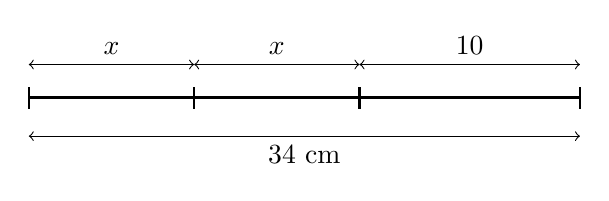
\begin{tikzpicture}[scale=0.7]
  \draw[thick] (0,0) -- (10,0);
  \draw[thick] (0,-0.2) -- (0,0.2);
  \draw[thick] (3,-0.2) -- (3,0.2);
  \draw[thick] (6,-0.2) -- (6,0.2);
  \draw[thick] (10,-0.2) -- (10,0.2);
  \draw[<->] (0,-0.7) -- (10,-0.7);
  \node[below] at (5,-0.7) {$34$ cm};
  \draw[<->] (0,0.6) -- (3,0.6);
  \node[above] at (1.5,0.6) {$x$};
  \draw[<->] (3,0.6) -- (6,0.6);
  \node[above] at (4.5,0.6) {$x$};
  \draw[<->] (6,0.6) -- (10,0.6);
  \node[above] at (8,0.6) {$10$};
\end{tikzpicture}
\end{center}
\end{questionText}
\choiceA{$3x = 34$}
\choiceB{$x + 10 = 34$}
\choiceC{$2x + 10 = 34$}
\choiceD{$2x - 10 = 34$}
\correctAnswer{C}
\explanation{The total length is two segments of $x$ plus one segment of $10$: $2x + 10 = 34$.}
\end{practiceQuestion}

\begin{practiceQuestion}{5-1-q29}{gsa}
\begin{questionText}
The diagram shows the perimeter of a rectangle. Write an equation that can be used to find $w$.

\begin{center}
\begin{tikzpicture}[scale=0.6]
  \draw[thick,fill=funBlue!10] (0,0) rectangle (6,3);
  \draw[<->] (0,-0.5) -- (6,-0.5);
  \node[below] at (3,-0.5) {$9$ cm};
  \draw[<->] (-0.5,0) -- (-0.5,3);
  \node[left] at (-0.5,1.5) {$w$ cm};
  \node at (3,4) {Perimeter $= 32$ cm};
\end{tikzpicture}
\end{center}
\end{questionText}
\correctAnswer{$2w + 18 = 32$ or $2(9) + 2w = 32$}
\explanation{Perimeter $= 2 \times 9 + 2w = 18 + 2w$. Set equal to $32$: $2w + 18 = 32$.}
\end{practiceQuestion}

\begin{practiceQuestion}{5-1-q30}{gsa}
\begin{questionText}
The table shows how much a dog-grooming service charges. Write an equation relating the total cost $C$ to the number of dogs $d$.

\begin{center}
\begin{tabular}{|c|c|}
\hline
\textbf{Dogs ($d$)} & \textbf{Cost ($C$)} \\
\hline
$1$ & $\$28$ \\
\hline
$2$ & $\$46$ \\
\hline
$3$ & $\$64$ \\
\hline
$5$ & $\$100$ \\
\hline
\end{tabular}
\end{center}
\end{questionText}
\correctAnswer{$C = 18d + 10$}
\explanation{Each dog adds $\$18$ ($46 - 28 = 18$). When $d = 1$: $18(1) + 10 = 28$ \checkmark. The equation is $C = 18d + 10$.}
\end{practiceQuestion}
